\documentclass[11pt]{article}
\usepackage[margin=2cm]{geometry}
\usepackage{amsmath,amssymb}
\usepackage{xcolor}
\usepackage{tikz}
\usepackage{contour}
\usepackage{float}
\usepackage[backend=biber,style=authoryear]{biblatex}
\addbibresource{bibliography.bib}
\contourlength{1.2pt}

\setlength{\parindent}{0pt}
\setlength{\parskip}{0.5\baselineskip}

\title{Astrofísica Moderna\\[0.4em]
\large Experimento de Stern--Gerlach}
\author{Daniel Soto Villada}
\date{\today}

\begin{document}
\maketitle

\section{Experimento de Stern--Gerlach}
\begin{figure}[htbp]
    \centering
    \begin{tikzpicture}[>=stealth, scale=1.25, transform shape, every node/.style={font=\small}, x={(2cm,0cm)}, y={(0.8cm,0.6cm)}, z={(0cm,1.7cm)}]
        \coordinate (O) at (0,0,0);
        \coordinate (X) at (1.8,0,0);
        \coordinate (Y) at (0,1.35,0);
        \coordinate (Z) at (0,0,1.45);
        \coordinate (S) at (1.8,1.35,1.45);

        \draw[->,gray!75] (-1.55,0,0) -- (3.0,0,0) node[below right] {\contour{white}{$x$}};
        \draw[->,gray!75] (0,-1.3,0) -- (0,2.15,0) node[above left] {\contour{white}{$y$}};
        \draw[->,gray!75] (0,0,-1.25) -- (0,0,2.05) node[above] {\contour{white}{$z$}};

        \draw[->,very thick,red!75!black] (O) -- (X)
            node[below right] at (X) {\contour{white}{$\vec{S}_x$}};
        \draw[->,very thick,blue!75!black] (O) -- (Y)
            node[above left] at (Y) {\contour{white}{$\vec{S}_y$}};
        \draw[->,very thick,green!55!black] (O) -- (Z)
            node[left] at (Z) {\contour{white}{$\vec{S}_z$}};
        \draw[densely dashed,gray!80] (X) -- (1.8,1.35,0) -- (S);
        \draw[densely dashed,gray!80] (Y) -- (1.8,1.35,0);
        \draw[densely dashed,gray!80] (Z) -- (S);
        \draw[->,ultra thick,black] (O) -- (S)
            node[above right] at (S) {\contour{white}{$\vec{S}$}};
        \draw[->,very thick,orange!85!black] (O) -- (-1.17,-0.8775,-0.9425)
            node[below left] at (-1.17,-0.8775,-0.9425) {\contour{white}{$\vec{\mu}_e$}};
        \filldraw[fill=white,draw=black,thick] (O) circle (0.18);
        \node[above left=2pt] at (O) {\contour{white}{$e^{-}$}};
    \end{tikzpicture}
    \caption{Esquema tridimensional de un electrón, el espín $\vec{S}$ y sus componentes $\vec{S}_x$, $\vec{S}_y$ y $\vec{S}_z$ en los ejes coordenados; el momento magnético $\vec{\mu}_e$ apunta en sentido opuesto, pues $\vec{\mu}_e=-g_e\mu_B\vec{S}/\hbar$, con $\mu_B=e\hbar/(2m_e)$. Para un electrón de espín $1/2$, cada componente medida puede tomar $S_i=\pm\hbar/2$. La descomposición dibujada es esquemática: las componentes no pueden medirse simultáneamente, ya que $[\hat S_i,\hat S_j]\ne0$ para $i\ne j$.}
    \label{fig:electron-sg}
\end{figure}
\begin{figure}[htbp]
    \centering
    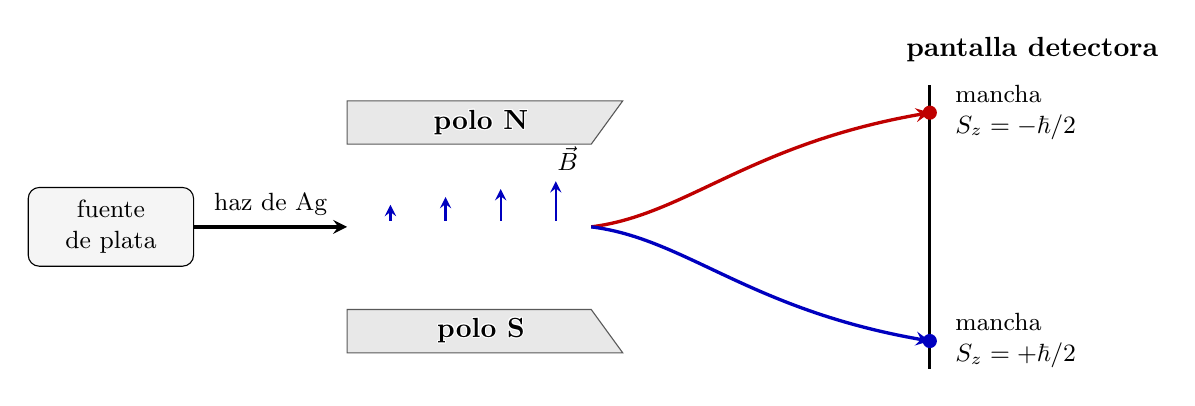
\begin{tikzpicture}[>=stealth, every node/.style={font=\small}]
        \node[draw,rounded corners,fill=gray!8,minimum width=2.1cm,minimum height=1cm,align=center] (source) at (1.0,0) {fuente\\de plata};
        \draw[->,very thick] (source.east) -- (4.0,0) node[midway,above] {\contour{white}{haz de Ag}};

        \draw[fill=gray!18,draw=gray!70!black] (4.0,1.6) -- (7.5,1.6) -- (7.1,1.05) -- (4.0,1.05) -- cycle;
        \draw[fill=gray!18,draw=gray!70!black] (4.0,-1.05) -- (7.1,-1.05) -- (7.5,-1.6) -- (4.0,-1.6) -- cycle;
        \node[font=\bfseries] at (5.7,1.32) {\contour{white}{polo N}};
        \node[font=\bfseries] at (5.7,-1.32) {\contour{white}{polo S}};
        \foreach \x/\h in {4.55/0.28,5.25/0.38,5.95/0.48,6.65/0.58} {
            \draw[->,blue!75!black,thick] (\x,0.08) -- (\x,\h);
        }
        \node[above] at (6.8,0.58) {\contour{white}{$\vec{B}$}};

        \draw[->,very thick,red!75!black] (7.1,0) .. controls (8.3,0.15) and (9.1,1.05) .. (11.4,1.45);
        \draw[->,very thick,blue!75!black] (7.1,0) .. controls (8.3,-0.15) and (9.1,-1.05) .. (11.4,-1.45);

        \draw[very thick] (11.4,-1.8) -- (11.4,1.8);
        \fill[red!75!black] (11.4,1.45) circle (0.09);
        \fill[blue!75!black] (11.4,-1.45) circle (0.09);
        \node[right,align=left] at (11.6,1.45) {\contour{white}{mancha}\\\contour{white}{$S_z=-\hbar/2$}};
        \node[right,align=left] at (11.6,-1.45) {\contour{white}{mancha}\\\contour{white}{$S_z=+\hbar/2$}};
        \node[font=\bfseries] at (12.7,2.25) {\contour{white}{pantalla detectora}};
    \end{tikzpicture}
    \caption{Esquema del experimento de Stern--Gerlach para átomos de plata en un campo inhomogéneo, con $\vec{B}=B_z\vec{e}_z$ y $\partial B_z/\partial z>0$. La fuerza es $\vec{F}=\mu_z(\partial B_z/\partial z)\vec{e}_z$; como el momento magnético del electrón $\vec{\mu}_e=-g_e\mu_B\vec{S}/\hbar$ es antiparalelo a su espín, los estados $S_z=\pm\hbar/2$ se desvían en sentidos opuestos.}
    \label{fig:sg-apparatus}
\end{figure}
\begin{enumerate}
    \item Al focalizar un haz de átomos de plata en un imán inhomogéneo, ¿qué patrón se observa en la pantalla?
    \begin{itemize}
        \item (A) Una mancha continua.
        \item \textcolor{red}{(B) Dos manchas discretas.}
        \item (C) Tres manchas simétricas.
        \item (D) Ninguna desviación.
    \end{itemize}
    \textit{Solución.} Clásicamente, las orientaciones aleatorias del momento magnético producirían un continuo de desviaciones. En el experimento se observan dos componentes discretas, asociadas a los dos valores permitidos de la proyección del momento magnético sobre el eje del imán. La respuesta es \textbf{(B)} (véase la Fig. \ref{fig:sg-apparatus}). \parencite[Sec. 18.2, pp. 581--582]{chaparro2026}

    \item La aparición de solo dos manchas en el experimento de Stern--Gerlach indica que la componente del espín electrónico sobre el eje $z$:
    \begin{itemize}
        \item (A) Es puramente orbital.
        \item (B) Se alinea con cualquier ángulo y produce un continuo de valores.
        \item (C) Depende de la velocidad de los átomos.
        \item \textcolor{red}{(D) Está cuantizada: $S_z=\pm\hbar/2$.}
    \end{itemize}
    \textit{Solución.} El sistema es de espín $1/2$, por lo que una medición de la componente $S_z$ solo puede dar los valores $+\hbar/2$ o $-\hbar/2$. Estos dos resultados explican las dos manchas observadas. La respuesta es \textbf{(D)} (véase la Fig. \ref{fig:electron-sg}). \parencite[Sec. 18.2, pp. 582--583]{chaparro2026}

    \item En un átomo de plata, la componente $\mu_z$ del momento magnético es proporcional a:
    \begin{itemize}
        \item (A) La masa del átomo.
        \item (B) El campo magnético externo.
        \item (C) La densidad de átomos del haz.
        \item \textcolor{red}{(D) La componente $S_z$ del espín del electrón de valencia no apareado.}
    \end{itemize}
    \textit{Solución.} El átomo de plata tiene sus capas internas cerradas y un electrón de valencia no apareado. Su momento angular orbital neto es cero, de modo que el momento magnético relevante se debe al espín de ese electrón. En particular, $\boldsymbol{\mu}_e=-g_e\mu_B\mathbf{S}/\hbar$, con $\mu_B=e\hbar/(2m_e)$; por ello, $\mu_z$ es proporcional a $S_z$ (con signo opuesto para el electrón). La respuesta es \textbf{(D)} (véase la Fig. \ref{fig:electron-sg}). \parencite[Sec. 18.2, pp. 581--583]{chaparro2026}

    \item Si el gradiente del campo magnético del aparato Stern--Gerlach está dirigido según $x$, ¿en cuántos componentes se separa el haz de átomos de plata?
    \begin{itemize}
        \item \textcolor{red}{(A) En dos componentes, $S_x=+\hbar/2$ y $S_x=-\hbar/2$.}
        \item (B) En cinco componentes.
        \item (C) En una franja central.
        \item (D) En un continuo clásico.
    \end{itemize}
    \textit{Solución.} El gradiente en $x$ mide la proyección del espín sobre ese eje. Para un sistema de espín $1/2$, los únicos resultados posibles son $S_x=\pm\hbar/2$, por lo que aparecen dos componentes. La respuesta es \textbf{(A)} (véase la Fig. \ref{fig:sg-x}). \parencite[Secs. 18.2.1 y 18.2.3, pp. 583--585, 593--595]{chaparro2026}
    \begin{figure}[htbp]
    \centering
    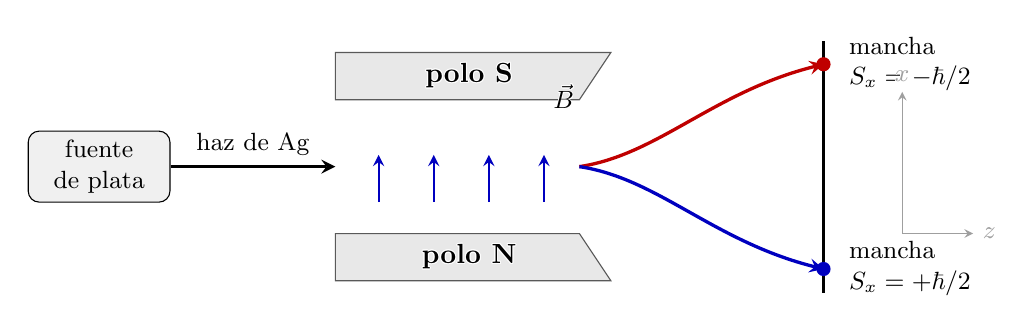
\begin{tikzpicture}[>=stealth, every node/.style={font=\small}]
        \node[draw,rounded corners,fill=gray!12,minimum width=1.8cm,minimum height=0.9cm,align=center] (source) at (0,0) {fuente\\de plata};
        \draw[->,very thick] (source.east) -- (3.0,0) node[midway,above] {\contour{white}{haz de Ag}};

        \draw[fill=gray!18,draw=gray!70!black] (3.0,1.45) -- (6.5,1.45) -- (6.1,0.85) -- (3.0,0.85) -- cycle;
        \draw[fill=gray!18,draw=gray!70!black] (3.0,-0.85) -- (6.1,-0.85) -- (6.5,-1.45) -- (3.0,-1.45) -- cycle;
        \node[font=\bfseries] at (4.7,1.15) {\contour{white}{polo S}};
        \node[font=\bfseries] at (4.7,-1.15) {\contour{white}{polo N}};
        \foreach \z in {3.55,4.25,4.95,5.65} {
            \draw[->,blue!75!black,thick] (\z,-0.45) -- (\z,0.15);
        }
        \node[above] at (5.9,0.6) {\contour{white}{$\vec{B}$}};

        \draw[->,very thick,red!75!black] (6.1,0) .. controls (7.1,0.15) and (7.8,0.95) .. (9.2,1.3);
        \draw[->,very thick,blue!75!black] (6.1,0) .. controls (7.1,-0.15) and (7.8,-0.95) .. (9.2,-1.3);
        \draw[very thick] (9.2,-1.6) -- (9.2,1.6);
        \fill[red!75!black] (9.2,1.3) circle (0.09);
        \fill[blue!75!black] (9.2,-1.3) circle (0.09);
        \node[right,align=left] at (9.4,1.3) {\contour{white}{mancha}\\\contour{white}{$S_x=-\hbar/2$}};
        \node[right,align=left] at (9.4,-1.3) {\contour{white}{mancha}\\\contour{white}{$S_x=+\hbar/2$}};
        \draw[->,gray!75] (10.2,-0.85) -- (10.2,0.95) node[above] {\contour{white}{$x$}};
        \draw[->,gray!75] (10.2,-0.85) -- (11.1,-0.85) node[right] {\contour{white}{$z$}};
    \end{tikzpicture}
    \caption{Analizador Stern--Gerlach con gradiente en la dirección $x$: $\vec{B}=B_x\vec{e}_x$ y $\partial B_x/\partial x>0$. La fuerza $\vec{F}=\mu_x(\partial B_x/\partial x)\vec{e}_x$ separa el haz según $S_x=\pm\hbar/2$; para el electrón, $\vec{\mu}_e$ es antiparalelo a $\vec{S}$.}
    \label{fig:sg-x}
\end{figure}

    \item Se bloquea el canal $S_z=-\hbar/2$ y se deja pasar el canal $S_z=+\hbar/2$ de un primer aparato $SG_z$. El haz transmitido entra en un segundo aparato $SG_z$. ¿Cuántos haces salen del segundo aparato?
    \begin{itemize}
        \item (A) Una distribución continua.
        \item (B) Tres haces.
        \item (C) Dos haces $S_z=\pm\hbar/2$ de igual intensidad.
        \item \textcolor{red}{(D) Un solo haz $S_z=+\hbar/2$.}
    \end{itemize}
    \textit{Solución.} El primer aparato, junto con el bloqueo del canal negativo, prepara el haz en un estado propio de $S_z$ con valor $+\hbar/2$. Una nueva medición sobre el mismo eje da ese mismo valor, así que el segundo aparato no divide el haz. La respuesta es \textbf{(D)} (véase la Fig. \ref{fig:secuencia-sg}). \parencite[Sec. 18.2.1, pp. 583--584]{chaparro2026}

    \item Se selecciona el canal $S_z=+\hbar/2$ de un aparato $SG_z$ y se envía a un aparato $SG_x$. ¿Cuántos haces resultan en la salida de $SG_x$?
    \begin{itemize}
        \item (A) Una distribución continua.
        \item (B) Tres haces.
        \item \textcolor{red}{(C) Dos haces $S_x=\pm\hbar/2$ de igual intensidad.}
        \item (D) Un solo haz $S_x=+\hbar/2$.
    \end{itemize}
    \textit{Solución.} El estado con $S_z=+\hbar/2$ es una superposición de los estados propios de $S_x$, con amplitudes de igual magnitud. Por la regla de Born, cada resultado $S_x=+\hbar/2$ y $S_x=-\hbar/2$ tiene probabilidad $1/2$. La respuesta es \textbf{(C)} (véase la Fig. \ref{fig:secuencia-sg}). \parencite[Secs. 18.2.1, 18.2.3 y 18.2.4, pp. 584, 593--596]{chaparro2026}

    \item En la secuencia $SG_z\to SG_x\to SG_z$, se selecciona el canal $S_x=+\hbar/2$ del segundo aparato. ¿Cuántos haces salen del tercer aparato $SG_z$?
    \begin{itemize}
        \item (A) Una distribución continua.
        \item (B) Tres haces.
        \item \textcolor{red}{(C) Dos haces $S_z=\pm\hbar/2$ de igual intensidad.}
        \item (D) Un solo haz $S_z=+\hbar/2$.
    \end{itemize}
    \textit{Solución.} Al seleccionar $S_x=+\hbar/2$, el haz queda preparado en un estado propio de $S_x$, que es una superposición equiprobable de los estados $S_z=+\hbar/2$ y $S_z=-\hbar/2$. El tercer aparato produce ambos haces con igual intensidad. La respuesta es \textbf{(C)} (véase la Fig. \ref{fig:secuencia-sg}). \parencite[Secs. 18.2.1, 18.2.3 y 18.2.4, pp. 585, 593--596]{chaparro2026}

    \item En la secuencia $SG_z\to SG_x\to SG_z$, el tercer aparato vuelve a mostrar ambos resultados $S_z=\pm\hbar/2$, aunque el primero había seleccionado $S_z=+\hbar/2$. Esto ilustra:
    \begin{itemize}
        \item (A) La conservación de $S_z$ a través de cualquier medición.
        \item \textcolor{red}{(B) La no conmutatividad de $S_x$ y $S_z$.}
        \item (C) La ley de Faraday.
        \item (D) La dualidad onda-partícula.
    \end{itemize}
    \textit{Solución.} Las componentes del espín sobre ejes distintos son observables incompatibles: $[\hat S_x,\hat S_z]\ne0$. Medir y seleccionar un resultado de $S_x$ modifica la preparación anterior de $S_z$; al medir $S_z$ de nuevo, aparecen ambos resultados. La respuesta es \textbf{(B)} (véase la Fig. \ref{fig:secuencia-sg}). \parencite[Sec. 18.2.5, p. 597]{chaparro2026}
    \begin{figure}[htbp]
    \centering
    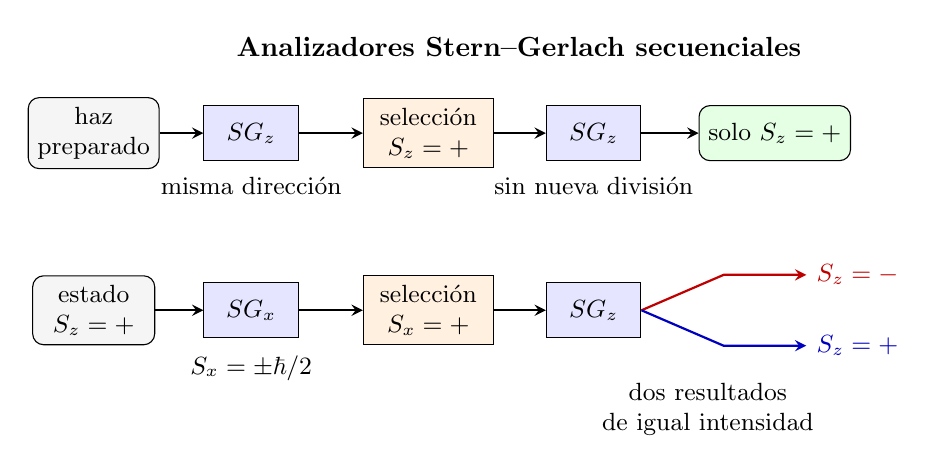
\begin{tikzpicture}[>=stealth, every node/.style={font=\small}]
        \node[font=\bfseries] at (5.4,2.15) {Analizadores Stern--Gerlach secuenciales};

        \node[draw,rounded corners,fill=gray!8,align=center,minimum width=1.55cm,minimum height=0.7cm] (source) at (0,1.05) {haz\\preparado};
        \node[draw,fill=blue!10,align=center,minimum width=1.2cm,minimum height=0.7cm] (sgz1) at (2.0,1.05) {$SG_z$};
        \node[draw,fill=orange!12,align=center,minimum width=1.65cm,minimum height=0.7cm] (selectz) at (4.25,1.05) {selección\\$S_z=+$};
        \node[draw,fill=blue!10,align=center,minimum width=1.2cm,minimum height=0.7cm] (sgz2) at (6.35,1.05) {$SG_z$};
        \node[draw,rounded corners,fill=green!10,align=center,minimum width=1.65cm,minimum height=0.7cm] (one) at (8.65,1.05) {solo $S_z=+$};
        \draw[->,thick] (source) -- (sgz1);
        \draw[->,thick] (sgz1) -- (selectz);
        \draw[->,thick] (selectz) -- (sgz2);
        \draw[->,thick] (sgz2) -- (one);
        \node[below] at (2.0,0.62) {misma dirección};
        \node[below] at (6.35,0.62) {sin nueva división};

        \node[draw,rounded corners,fill=gray!8,align=center,minimum width=1.55cm,minimum height=0.7cm] (prepared) at (0,-1.2) {estado\\$S_z=+$};
        \node[draw,fill=blue!10,align=center,minimum width=1.2cm,minimum height=0.7cm] (sgx) at (2.0,-1.2) {$SG_x$};
        \node[draw,fill=orange!12,align=center,minimum width=1.65cm,minimum height=0.7cm] (selectx) at (4.25,-1.2) {selección\\$S_x=+$};
        \node[draw,fill=blue!10,align=center,minimum width=1.2cm,minimum height=0.7cm] (sgz3) at (6.35,-1.2) {$SG_z$};
        \draw[->,thick] (prepared) -- (sgx);
        \draw[->,thick] (sgx) -- (selectx);
        \draw[->,thick] (selectx) -- (sgz3);
        \draw[->,thick,red!75!black] (sgz3.east) -- (8.0,-0.75) -- (9.05,-0.75) node[right] {$S_z=-$};
        \draw[->,thick,blue!75!black] (sgz3.east) -- (8.0,-1.65) -- (9.05,-1.65) node[right] {$S_z=+$};
        \node[below] at (2.0,-1.65) {$S_x=\pm\hbar/2$};
        \node[below,align=center] at (7.8,-2.0) {dos resultados\\de igual intensidad};
    \end{tikzpicture}
    \caption{Dos secuencias de analizadores: repetir una medición de $S_z$ conserva el resultado seleccionado; intercalar una medición de $S_x$ permite luego obtener ambos valores de $S_z$.}
    \label{fig:secuencia-sg}
\end{figure}

    \item ¿Qué ocurre al colocar dos polarizadores lineales cruzados, uno con eje de transmisión $x$ y otro con eje $y$, uno después del otro?
    \begin{itemize}
        \item (A) No se modifica la polarización.
        \item (B) Se duplica la intensidad.
        \item (C) Se transmite luz en $y$ aunque el primer filtro la haya cancelado.
        \item \textcolor{red}{(D) Se bloquea toda la luz.}
    \end{itemize}
    \textit{Solución.} Los ejes $x$ y $y$ son perpendiculares. La luz que sale del primer polarizador está polarizada en $x$ y su componente sobre el eje $y$ es nula; por tanto, el segundo polarizador no transmite luz. La respuesta es \textbf{(D)} (véase la Fig. \ref{fig:polarizadores}). \parencite[Sec. 18.2.2, pp. 586--589]{chaparro2026}

    \item Se coloca un polarizador con eje de transmisión a $45^\circ$ entre dos polarizadores cruzados, orientados en $x$ y $y$. ¿Qué ocurre?
    \begin{itemize}
        \item (A) No se modifica la polarización ni la intensidad.
        \item (B) Se duplica la intensidad.
        \item \textcolor{red}{(C) Se transmite una fracción no nula de luz a través del polarizador final en $y$.}
        \item (D) Se bloquea toda la luz, igual que sin el filtro intermedio.
    \end{itemize}
    \textit{Solución.} El filtro intermedio proyecta la polarización en una dirección que tiene componentes tanto en $x$ como en $y$. Por la ley de Malus, el primer filtro intermedio transmite la mitad de la intensidad y el filtro final transmite la mitad de esa cantidad: $I_{\mathrm{salida}}=I_{\mathrm{entrada}}\cos^2(45^\circ)\cos^2(45^\circ)=I_{\mathrm{entrada}}/4$. Por ello, se transmite luz aunque los polarizadores inicial y final estén cruzados. La respuesta es \textbf{(C)} (véase la Fig. \ref{fig:polarizadores}). \parencite[Sec. 18.2.2, pp. 588--592]{chaparro2026}
    \begin{figure}[htbp]
    \centering
    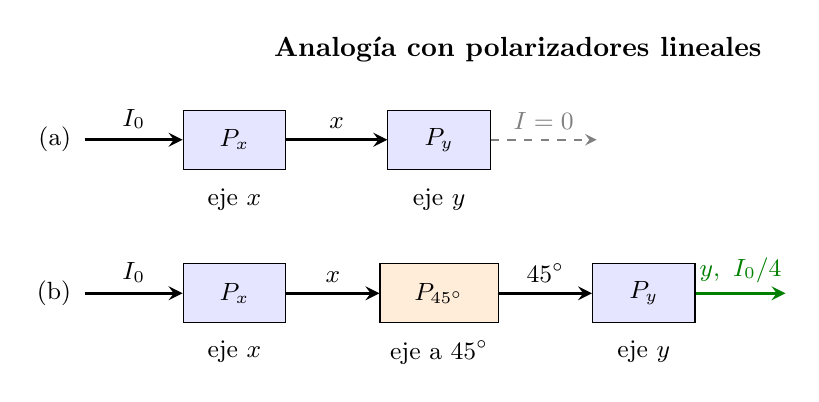
\begin{tikzpicture}[>=stealth, every node/.style={font=\small}]
        \node[font=\bfseries] at (5.0,2.0) {Analogía con polarizadores lineales};

        \node[draw,fill=blue!10,minimum width=1.3cm,minimum height=0.75cm] (x1) at (1.4,0.85) {$P_x$};
        \node[draw,fill=blue!10,minimum width=1.3cm,minimum height=0.75cm] (y1) at (4.0,0.85) {$P_y$};
        \draw[->,very thick] (-0.5,0.85) -- (x1.west) node[midway,above] {$I_0$};
        \draw[->,very thick] (x1.east) -- (y1.west) node[midway,above] {$x$};
        \draw[->,thick,dashed,gray] (y1.east) -- (6.0,0.85) node[midway,above] {$I=0$};
        \node[below] at (1.4,0.35) {eje $x$};
        \node[below] at (4.0,0.35) {eje $y$};
        \node[left] at (-0.55,0.85) {(a)};

        \node[draw,fill=blue!10,minimum width=1.3cm,minimum height=0.75cm] (x2) at (1.4,-1.1) {$P_x$};
        \node[draw,fill=orange!15,minimum width=1.5cm,minimum height=0.75cm] (d45) at (4.0,-1.1) {$P_{45^\circ}$};
        \node[draw,fill=blue!10,minimum width=1.3cm,minimum height=0.75cm] (y2) at (6.6,-1.1) {$P_y$};
        \draw[->,very thick] (-0.5,-1.1) -- (x2.west) node[midway,above] {$I_0$};
        \draw[->,very thick] (x2.east) -- (d45.west) node[midway,above] {$x$};
        \draw[->,very thick] (d45.east) -- (y2.west) node[midway,above] {$45^\circ$};
        \draw[->,very thick,green!50!black] (y2.east) -- (8.4,-1.1) node[midway,above] {$y,\ I_0/4$};
        \node[below] at (1.4,-1.58) {eje $x$};
        \node[below] at (4.0,-1.58) {eje a $45^\circ$};
        \node[below] at (6.6,-1.58) {eje $y$};
        \node[left] at (-0.55,-1.1) {(b)};
    \end{tikzpicture}
    \caption{Polarizadores cruzados bloquean la luz, pero un polarizador intermedio a $45^\circ$ transmite una fracción no nula ($I_0/4$) a través del último filtro.}
    \label{fig:polarizadores}
\end{figure}

    \item El estado $|S_x;+\rangle$ expresado como combinación de los estados $|S_z;+\rangle$ y $|S_z;-\rangle$ tiene coeficientes:
    \begin{itemize}
        \item (A) $1$ y $0$.
        \item (B) $1/2$ y $1/2$.
        \item \textcolor{red}{(C) $1/\sqrt{2}$ y $1/\sqrt{2}$.}
        \item (D) Complejos arbitrarios.
    \end{itemize}
    \textit{Solución.} En la base de autoestados de $S_z$, el estado con espín positivo en $x$ es
    \[
        |S_x;+\rangle=\frac{1}{\sqrt{2}}|S_z;+\rangle+\frac{1}{\sqrt{2}}|S_z;-\rangle.
    \]
    Por tanto, los dos coeficientes son $1/\sqrt{2}$ y $1/\sqrt{2}$. La respuesta es \textbf{(C)} (véase la Fig. \ref{fig:superposicion-spin}). \parencite[Sec. 18.2.3, pp. 594--595]{chaparro2026}
    \begin{figure}[H]
    \centering
    \begin{tikzpicture}[>=stealth, scale=1.1, transform shape, every node/.style={font=\small}, x={(2cm,0cm)}, y={(0cm,2cm)}]
        \coordinate (O) at (0,0);
        \coordinate (Zplus) at (0,1.35);
        \coordinate (Zminus) at (1.35,0);
        \coordinate (State) at (1.35,1.35);

        \draw[->,gray!75] (O) -- (0,1.85) node[above] {\contour{white}{$|S_z;+\rangle$}};
        \draw[->,gray!75] (O) -- (1.85,0) node[right] {\contour{white}{$|S_z;-\rangle$}};
        \draw[densely dashed,gray] (Zplus) -- (State) -- (Zminus);
        \draw[->,very thick,blue!75!black] (O) -- (State)
            node[above right] at (State) {\contour{white}{$|S_x;+\rangle$}};
        \node[left] at (Zplus) {\contour{white}{$1/\sqrt{2}$}};
        \node[below] at (Zminus) {\contour{white}{$1/\sqrt{2}$}};
        \fill (O) circle (0.04);
    \end{tikzpicture}
    \caption{Representación de las amplitudes de $|S_x;+\rangle$ en la base de $S_z$: $|S_x;+\rangle=(|S_z;+\rangle+|S_z;-\rangle)/\sqrt{2}$. Las dos amplitudes tienen módulo $1/\sqrt{2}$, por lo que cada resultado de una medición de $S_z$ tiene probabilidad $1/2$.}
    \label{fig:superposicion-spin}
\end{figure}
\end{enumerate}

\printbibliography[title={Referencias}]

\end{document}